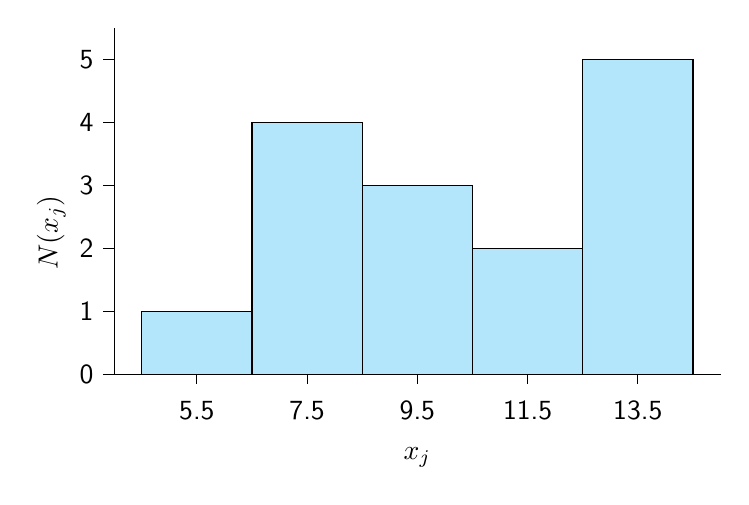
\begin{tikzpicture}[x=0.7cm, y=0.8cm, font=\sffamily]
    \draw (4,0) -- (15,0);
    \draw (4,0) -- (4,5.5);
    \foreach \y in {0,1,2,3,4,5} {
      \draw (4,\y) -- (3.8,\y) node[left] {\y};
    }
    \node[left=0.8cm, rotate=90] at (4,3) {$N(x_j)$};
    \foreach \x in {5.5, 7.5, 9.5, 11.5, 13.5} {
      \draw (\x,0) -- (\x,-0.15) node[below=0.1cm] {\x};
    }
    \node[below=0.8cm] at (9.5,0) {$x_j$};
    \draw[fill=cyan!30] (4.5,0) rectangle (6.5,1);
    \draw[fill=cyan!30] (6.5,0) rectangle (8.5,4);
    \draw[fill=cyan!30] (8.5,0) rectangle (10.5,3);
    \draw[fill=cyan!30] (10.5,0) rectangle (12.5,2);
    \draw[fill=cyan!30] (12.5,0) rectangle (14.5,5);
  \end{tikzpicture}